\documentclass[12pt,journal]{IEEEtran}

\usepackage{footmisc}
\usepackage[hidelinks]{hyperref}
\usepackage[T1]{fontenc}
\usepackage[utf8]{inputenc}
\usepackage{listings}
\usepackage{graphicx}
\usepackage{dblfloatfix}
\usepackage{caption}
\usepackage{minted}
\usepackage{bookmark}
\captionsetup{font=footnotesize}

% Keywords command
\providecommand{\keywords}[1]
{
  \small	
  \textbf{\textit{Keywords---}} #1
}

\graphicspath{ {../images/} }
\begin{document}
\pagestyle{empty}
\title{Representing year plannings of teachers in RDF}
\author{Michiel Rogissart\\[12pt]
	\large Supervisor: Dr. ir. Ben de Meester, Prof. dr. Kris Coolsaet \\
	Counsellor: Thomas Delva}
\maketitle

\pagenumbering{roman}

\setcounter{page}{3}
\thispagestyle{plain}
\pagestyle{plain}
\begin{abstract}
One of the advantages of linked data is the fact that it allows insightful information about data, with less complex queries than for example SQL \cite{sqlvsqparql}.
This advantage can be exploited by teachers that want a good insight in their year plan. A year plan is the collection of all lessons a teacher gives throughout a shool year.
Keeping track of certain properties of lessons, like interactivity and covered goals, can be quite a challenge now.
As a result, not many teachers actually keep track of these properties.
Tools exist to help teachers, but they have some problems because of their centralized nature.\\
This research proposes a linked data model for modelling year plannings. The goal is to offer a lot of useful insights about year plannings, without burdening teachers with having to enter a lot of data themselves.
The model was created using the eXtreme Design methodology\cite{xd}. To achieve this, competency questions were deduced from interviews with domain experts.
Every competency question has a corresponding SPARQL query, implying that this model is functional for the use case.
\keywords{Linked data, Education, RDF Ontology}
\end{abstract}

\section{Introduction and objective}

\noindent The objective of this research is to develop a linked data model representing year plannings. This should be done based on the needs of teachers.
More specifically, it is important to identify important aspects of year plannings that can be presented in an uncluttered way to teachers. \\ \\
Granularity, data consistency and the reuse of existing ontologies are key concepts in developing this model to ensure a durable result.\\
An analysis of the existing tools, and what teachers think these lack, is also important. Especially the problems arising from the centralized nature.
In the next subsection, these exsiting tools and their problems are discussed.

\subsection{Existing tools}
\label{subsection:existing-tools}
\noindent Most existing educational tools focus on relieving teachers from their administrative duties by providing an interface to delegate, grade and keep track of assignments and tests for their pupils.
Tools like Google Classroom \footnote{https://edu.google.com/intl/ALL\_nl/workspace-for-education/classroom/} and Planboard \footnote{https://www.chalk.com/planboard/} provide this functionality.\\ \\
Another important tool, especially for Flemish education \cite{destandaard}, is Smartschool \footnote{https://www.smartschool.be/}.\\
This is an online learning platform that offers some functionality to maintain lesson preparations.\\ \\
Important problems recurring in these tools are listed in the following.
\begin{itemize}
	\item Functionality to link exercises/lessons with competencies is either limited or not present at all.
 	\item Because all data resides on servers owned by a single company, no one can use the tools when these servers fail. When they get hacked, the hackers have information about a lot of pupils.
	\item Most of these tools are made for North-American education: it is hardly usable for teachers outside the USA.
 	\item Not a lot of insightful information can be presented to the user. Usually only the covered competencies are presented. Properties like interactivity and used materials are usually not supported.
  	\item No, or limited, functionality to link lessons to their used educational materials.
   	\item The granularity is limited to lesson level. This means that it becomes tricky to move parts of lessons around when needed.
    \item Teachers need to enter most data themselves, rather than depending on different sources. A teacher shouldn't for example have to enter metadata about educational materials that was created by publishers. 
\end{itemize}

\section{Materials and Methodology}

\noindent In this section, the used materials and eXtreme Design method are discussed.

\subsection{Used materials}
\noindent The materials on which this model and data is based, are discussed here. Both existing ontologies and published data are used to achieve a functional model.

\subsubsection{Existing ontologies}
This model is primarily build using Schema.org \cite{schema}. This offers a lot of classes and properties for an educational context.
Especially the \textit{schema:CreativeWork} class is often used. \\
Educational material used in lessons (like text books) are modelled using DC \cite{dc} ontologies. More specifically bibo \cite{bibo} and dcterms \cite{dcterms}.
This because it offers more granularity in describing documents than Schema.org.\\ \\
These ontologies implement the IEEE standard \cite{ieeelom} concerning LOMs (Learning Object Metadata).

\subsubsection{Data sources}
The Flemish government released a skos dataset \cite{ilearnskosmos} describing competencies, educational levels and curricula within the Flemish educational system.
This was developed within the i-Learn project \footnote{https://www.i-learn.vlaanderen/}. \\
Another important result of the i-learn project is a standard vocabulary \cite{pubelovoc} to be used when describing LOMs.
They also propose a metadata profile \cite{pubelo} based on IEEE-LOM. \\ \\
Another data source worth mentioning is a JSON API \footnote{https://onderwijs-vlaanderen-portaalov.apigee.io/apis} released by the Flemish government, containing the same data as the skos dataset. This however is not communicated using linked data.

\subsection{Methodology}

\noindent The eXtreme Design methodology \cite{xd} was used to develop this model. This offers a road map for developing ontologies based on the needs of the user.
This roadmap is depicted in figure \ref{fig:xd-diagram}.

\begin{figure}
	\caption[Extreme Design roadmap]{Extreme Design roadmap as mentioned in \cite{xd}}
	\centering
	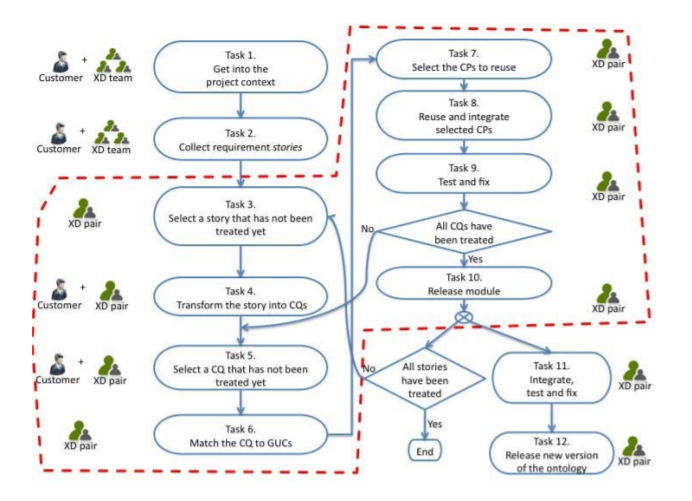
\includegraphics[scale=0.75]{xd-diagram.PNG}
	\label{fig:xd-diagram}
\end{figure}
\noindent To identify the needs of the user, interviews are conducted with domain experts. These interviews are processed into requirement stories: concrete stories on how one would use the model.\\
These requirement stories translate to competency questions. These are concrete questions a user might ask.
Contextual statements are added to aid developers in understanding the data (on which they are not an expert).\\
These competency questions are then implemented by augmenting the model and constructing SPARQL queries that answer them.

\section{Results and discussion}

\noindent The resulting model is discussed in this section. It is split up into different aspects to maintain an overview.

\subsection{Competencies}
\noindent Competencies are modelled as depicted in figure \ref{fig:uml-comp} .

\begin{figure}[h]
    \caption{Modelling of competencies}
    \label{fig:uml-comp}
    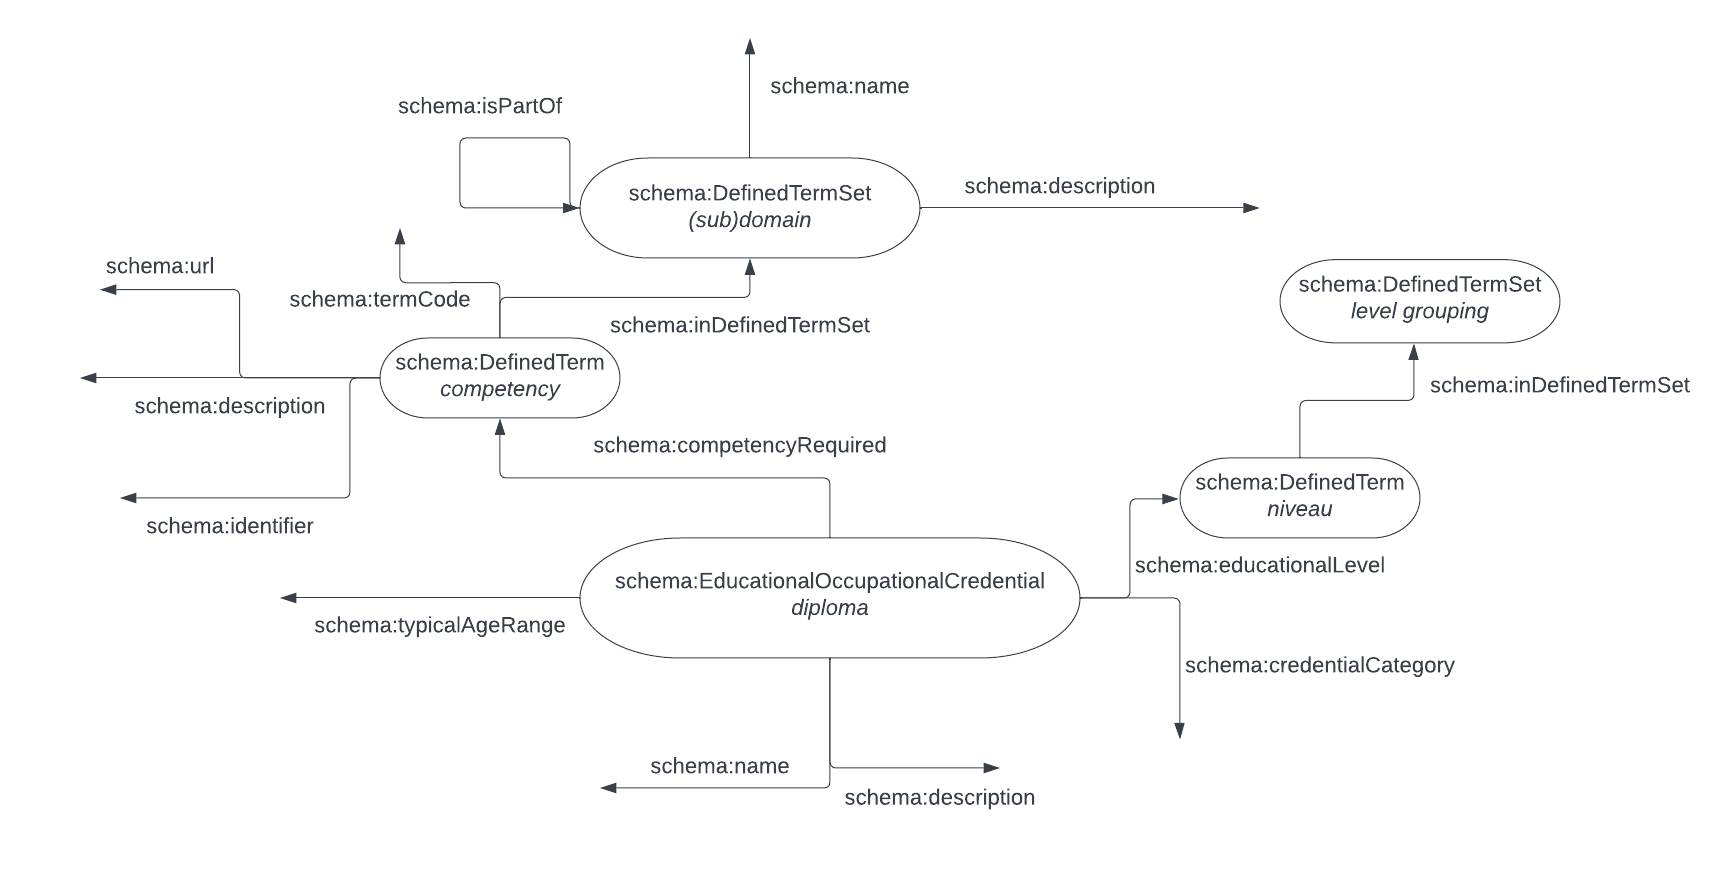
\includegraphics[scale=0.3]{uml-competencies.png}
\end{figure}
\noindent They are represented by the class \textit{schema:DefinedTerm}. This makes it independent of the ontology used by the government to release this data.\\
Competencies are typically grouped together in domains. This is done with the \textit{schema:DefinedTermSet} class.\\ \\
The educational level a pupil chose, is also modelled with \textit{schema:DefinedTerm} and can be grouped using \textit{schema:DefinedTermSet}.\\
Linking educational levels to their recquired competencies is done with \textit{schema:EducationalOccupationalCredential}, representing a diploma or certificate one can acquire.

\subsection{Year plannings}
\label{subsection:yearplan}
\noindent Year plannings are modelled as despicted in figure \ref{fig:uml-lesson}.
It is important to mention that these concepts do not contain temporal data.

\begin{figure}[h]
    \caption{Modelling of year plannings}
    \label{fig:uml-lesson}
    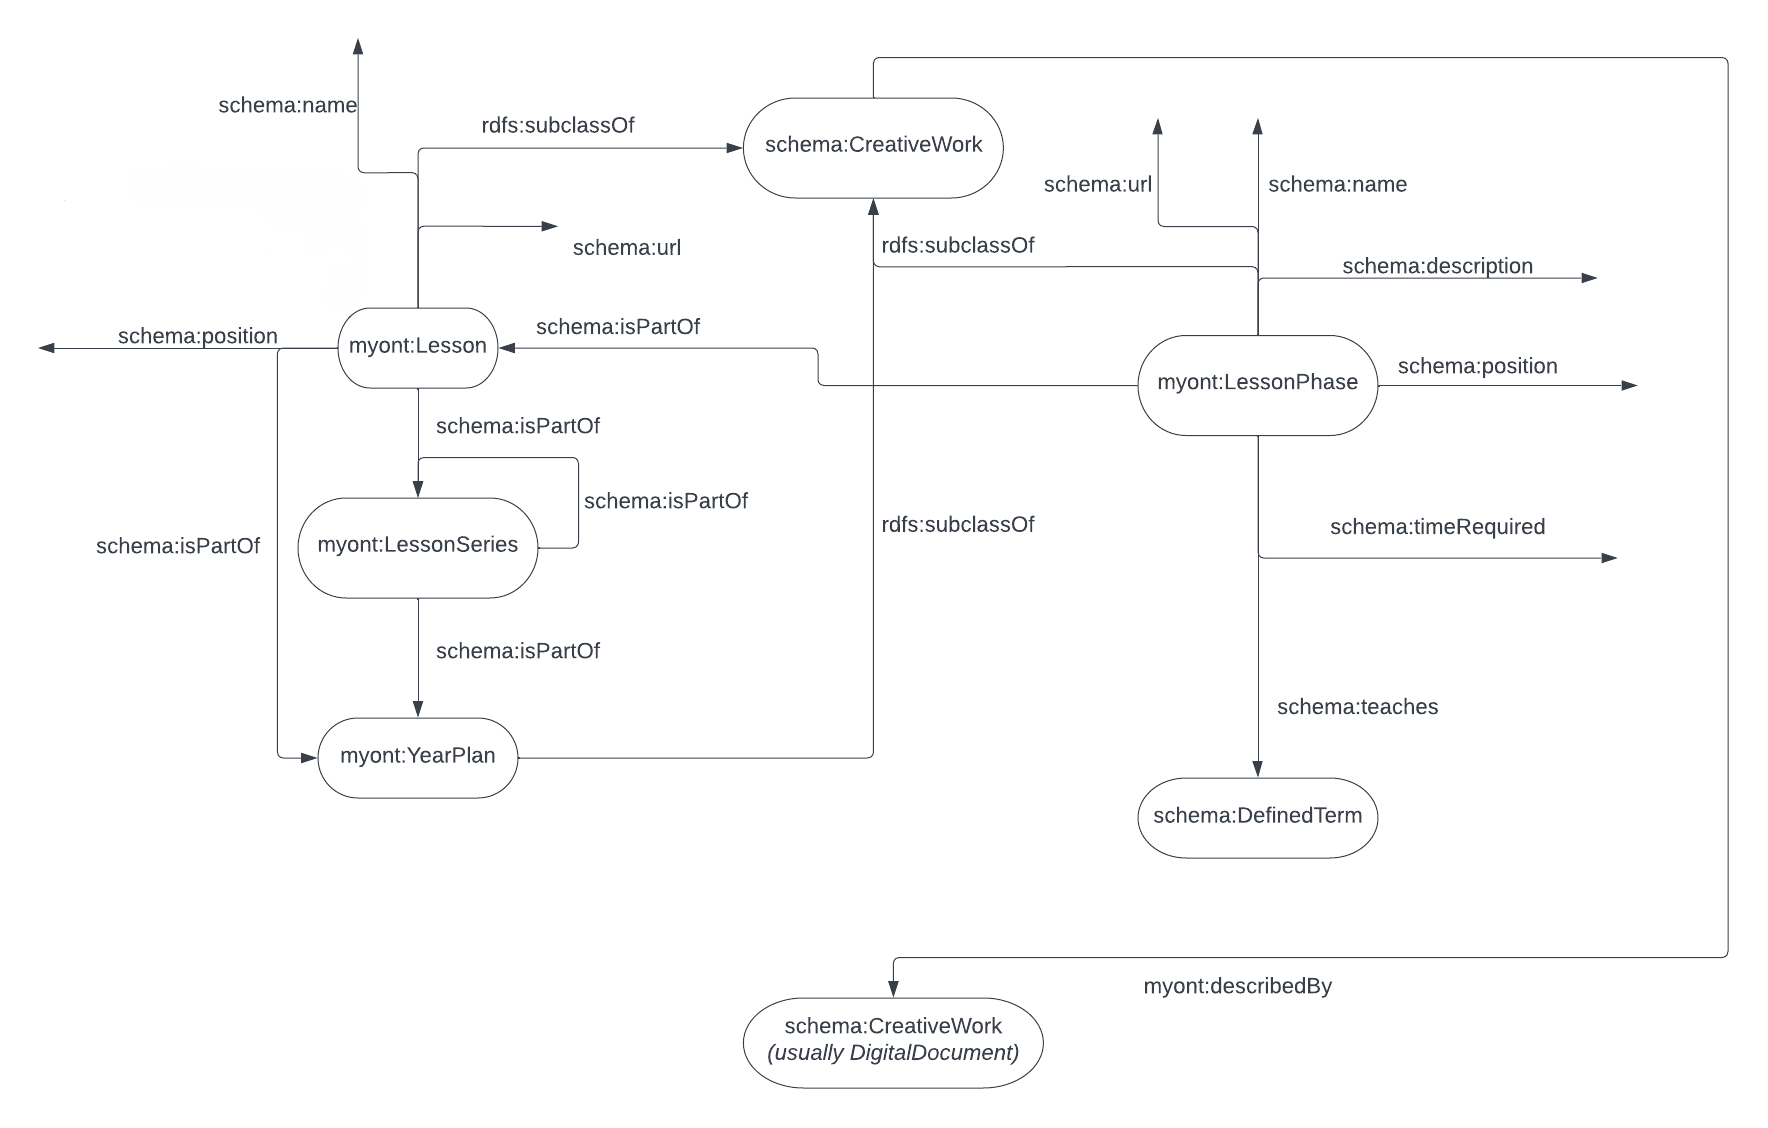
\includegraphics[scale=0.3]{uml-lessons.png}
\end{figure}
\noindent New classes are introduced because Schema.org didn't offer enough semantic distinctions between the different concepts.
All these classes inherit from \textit{schema:CreativeWork}.\\
To ensure granularity and data consistency, a hierarchy should be followed: lesson phases are part of lessons, lessons are part of lessons series and lesson series are part of a year plan.\\
To provide a flexible way of describing resources, every introduced class can have the \textit{myont:describedBy} property pointing to a document describing the phase, lesson...

\subsection{courses}
\noindent As mentioned, the concepts in subsection \ref{subsection:yearplan} do not contain temporal data.
To indicate when lessons are being taught, the model in figure \ref{fig:uml-courses} is used.

\begin{figure}[h]
	\caption{Modelling of courses}
	\label{fig:uml-courses}
	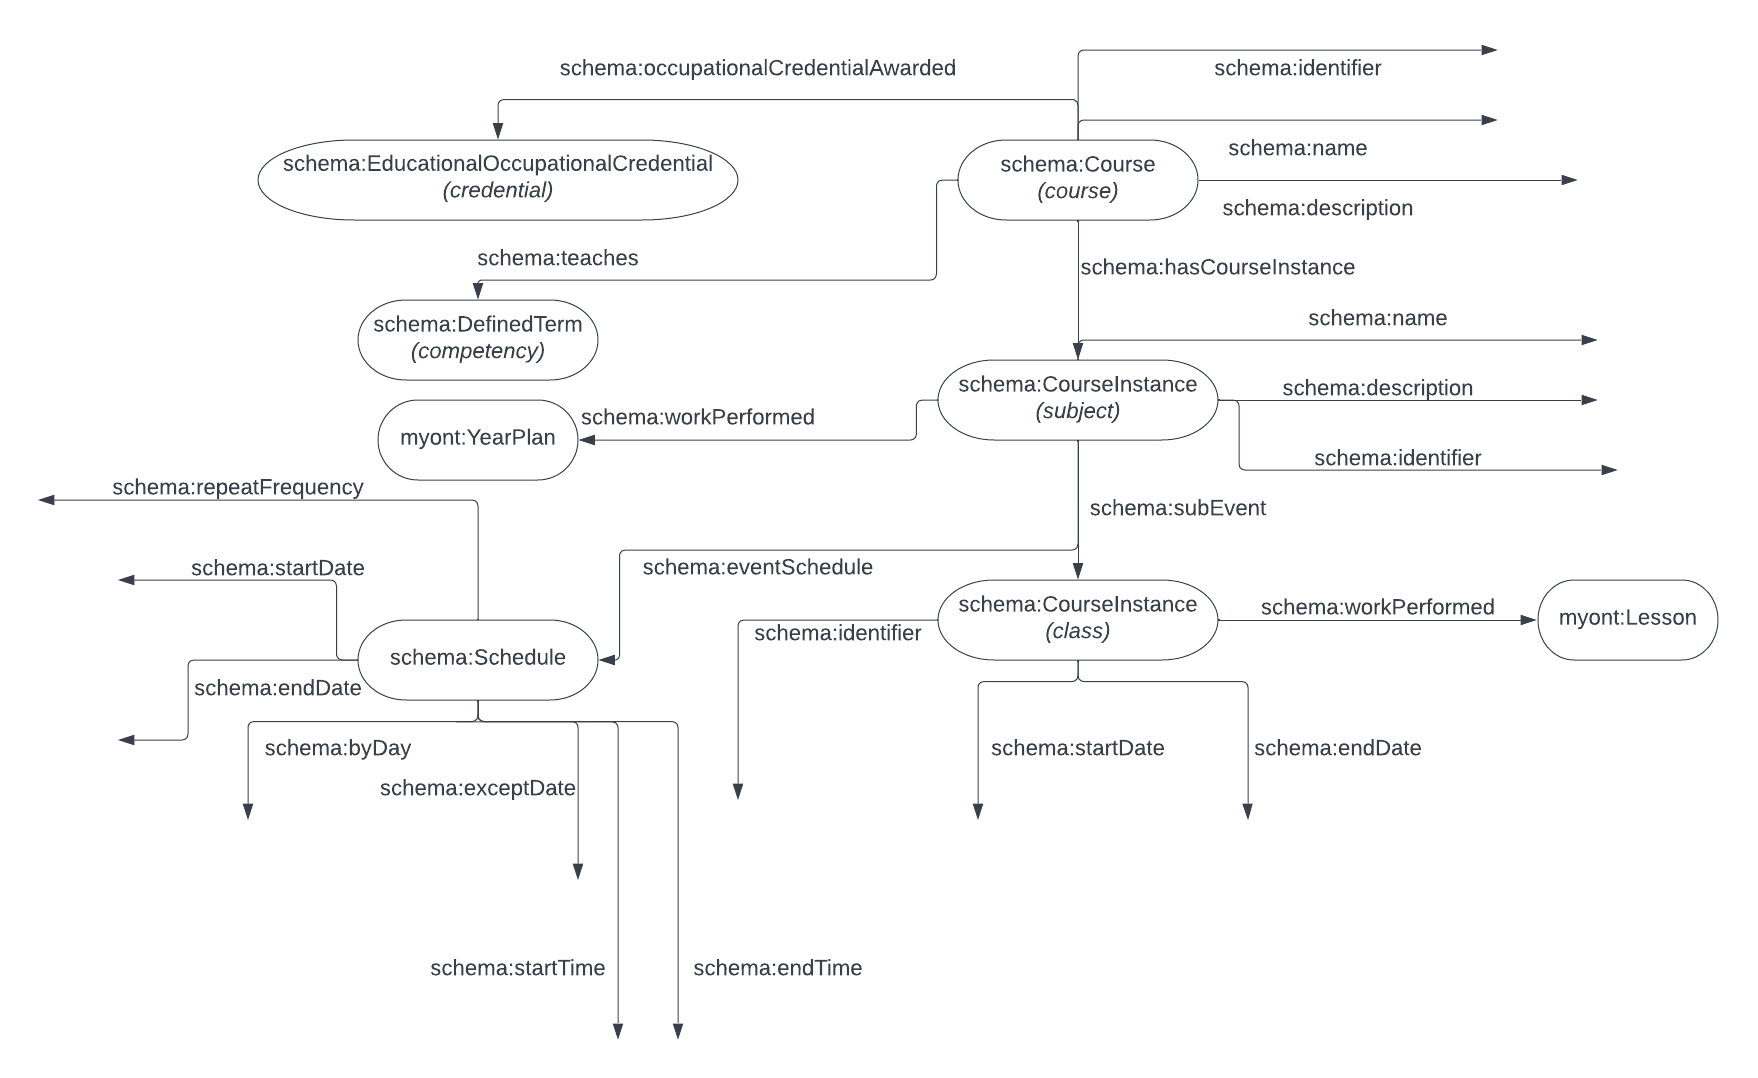
\includegraphics[scale=0.35]{uml-courses.png}
\end{figure}
\noindent A course is a set of competencies that is taught by a teacher to a group of students.
Subjects can be instantiated that add temporal data to a course. Subjects have a schedule indicating when classes occur.
Typically, a new subject will be created for every school year.
A class is a continous time period in which the teacher teaches a subset of the competencies that have to be taught in the course.\\
The term `class' is used to distinguish between lessons from subsection \ref{subsection:yearplan}, which contains no temporal data.
One year plan is taught within a subject, and one lesson is given during a class.

\subsection{Course materials and exercises}

\noindent Modelling course materials and exercises is done following the data model depicted in figure \ref{fig:uml-materialdata}.

\begin{figure}[h]
	\centering
	\caption{Modelling of course materials and exercises}
	\label{fig:uml-materialdata}
	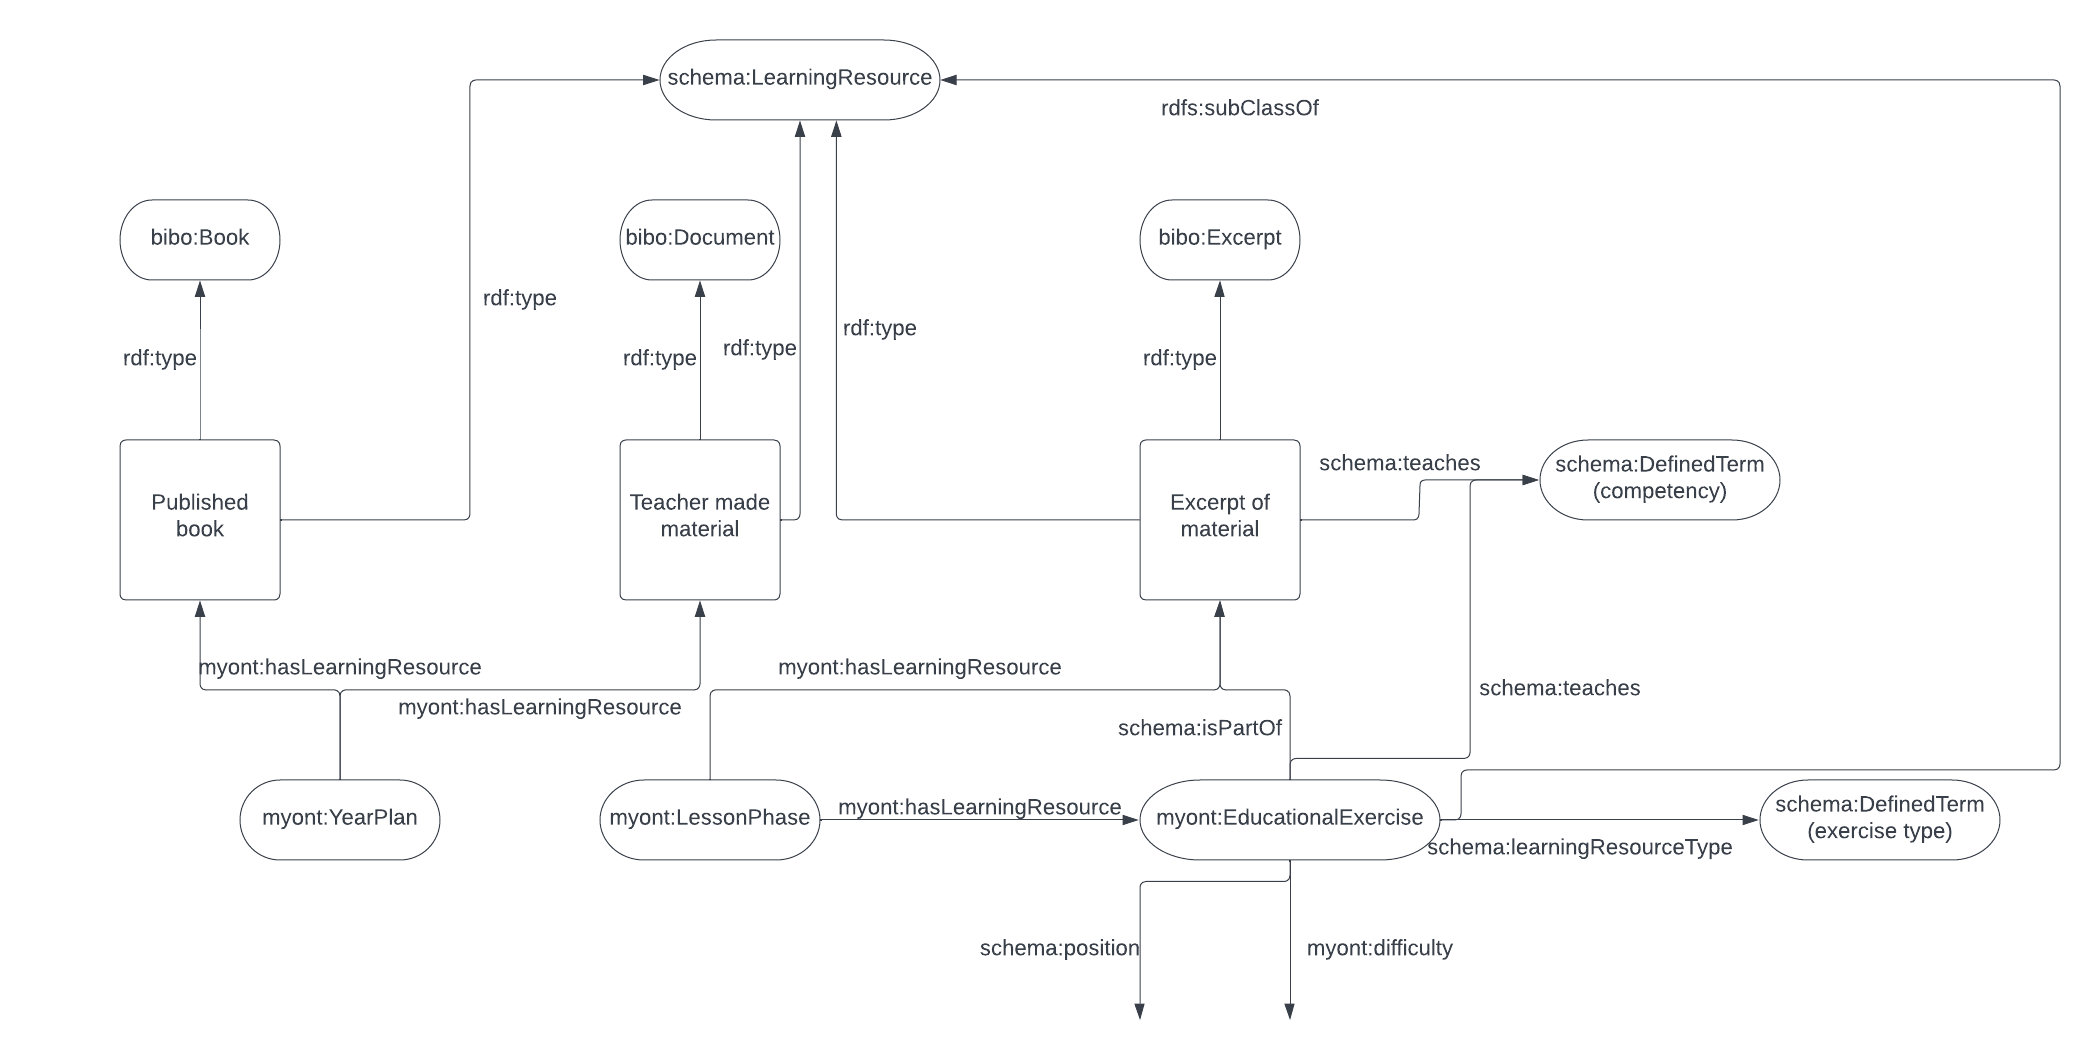
\includegraphics[scale=0.25]{uml-materialdata.png}
\end{figure}
\noindent All instances representing course material should have the type \textit{schema:LearningResource} in addition to a type of the bibo ontology.
This is needed because properties of both Schema.org and DC are used to describe these resources.\\
A new class representing educational exercises was introduced as Schema.org nor DC offered enough properties to describe these.

\subsection{Didactical methods and educational taxonomies}

\noindent A didactical method is the way one teaches subject matter.
The choice was made to not seperatly model these, but rather adding properties to existing classes representing important aspects as deduced from the interviews.
Modelling didactical methods is outside the scope of this research. A good reference for this is Mencke, S. et al \cite{hierarchy}.\\
Educational taxonomies are taxonomies indicating on which level one possesses the subject matter.
This is modelled using Schema.org, as shown in figure \ref{fig:uml-dm}.

\begin{figure}[h]
	\caption{Modelling of didactical methods and taxonomies}
	\label{fig:uml-dm}
	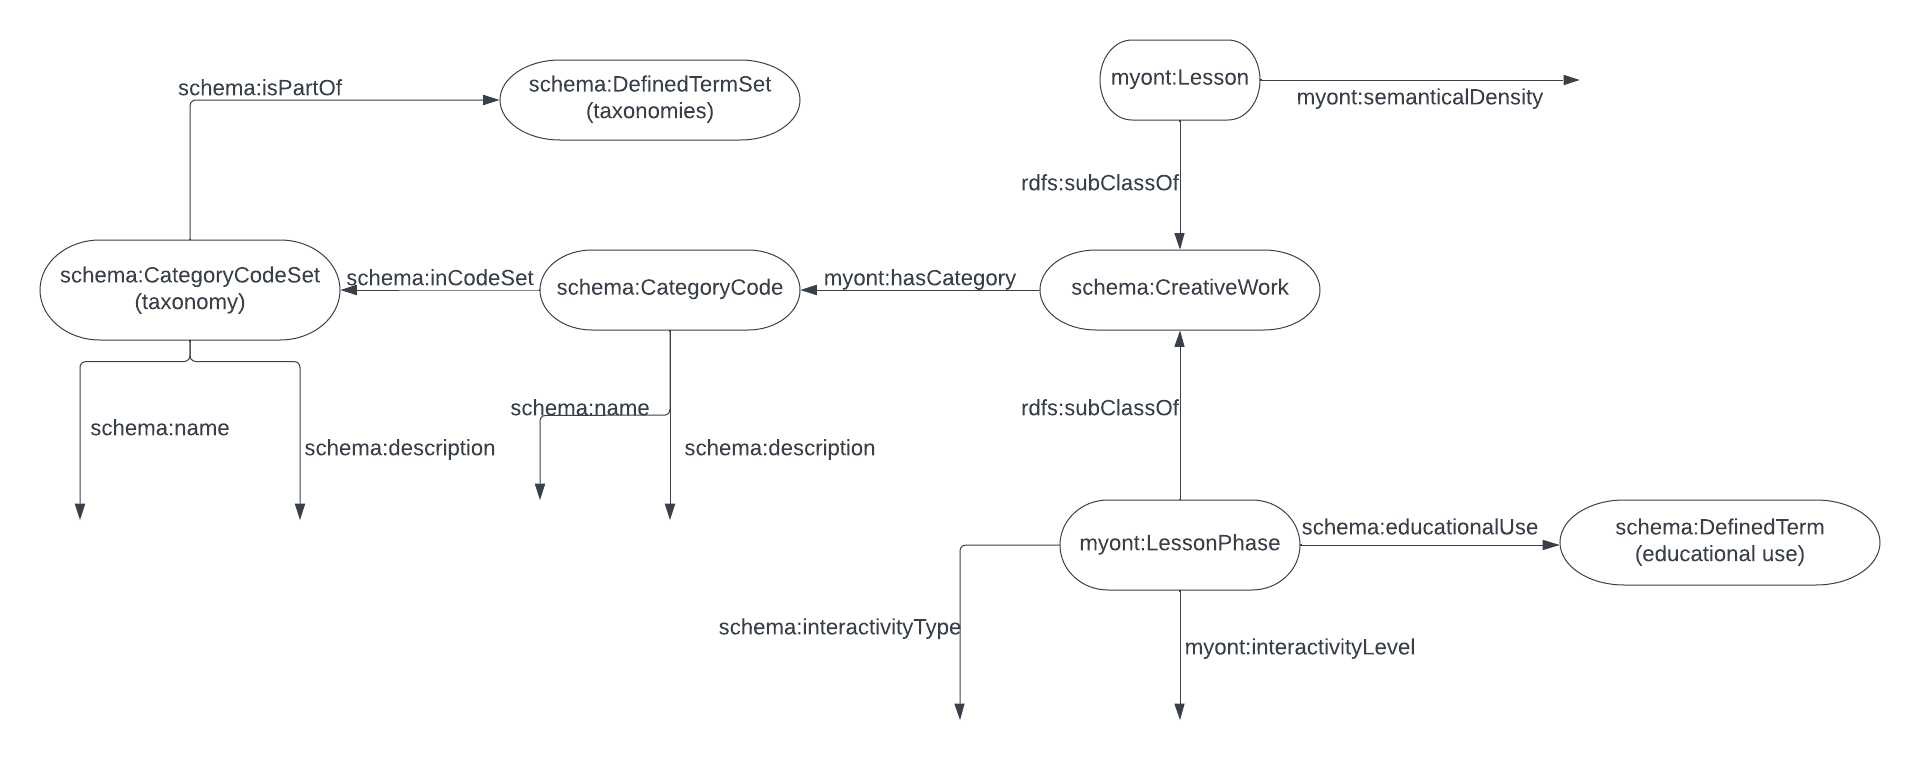
\includegraphics[scale=0.3]{uml-taxonomies.png}
\end{figure}

\section{Conclusion}

\noindent Most of the problems mentioned in section \ref{subsection:existing-tools} are solved because of the decentralized nature of linked data.
The data can be hosted by different companies, implying that if one company fails, only the teachers that store their data there are affected.
Switching companies will not mean loss of data.\\
Teachers also don't have to enter all data themselves because of this. Publishers can for example publish data about their text books.\\ \\
By modelling competencies as \textit{schema:DefinedTerm}, the official data of the government can be used without relying on the underlying ontology.
This means that this model is useable for every educational system based on competencies.\\ \\
By introducing \textit{myont:LessonPhase}, more granularity is provided. These phases can be moved around lessons when needed.\\
The competency questions taken out of the interviews, represent overviews the interviewees deemed useful.
By providing SPARQL queries, it is shown that these overviews can be offered to teachers.

\section*{ACKNOWLEDGMENTS}
\noindent I thank Thomas Delva and Dr. ir. Ben De Meester (University of Ghent) for their intensive guidance while developing this model.
Also a thanks to Prof. dr. Kris Coolsaet (University of Ghent) for helping with the educational part of the research.
The teachers giving me some of their free time to conduct an interview, are also thanked.\\
A special thanks to Prof. dr. ir. Ruben Verborgh (Univeristy of Ghent) for sparking my interest in linked data.

\bibliographystyle{IEEEtran}
\bibliography{../bibliography}

\end{document}